Hare and Hounds is a simple game with two players who alternate turns. One
player plays as the hare while the other plays as three hounds. The goal of the
hare is to escape the hounds while the goal of the hounds is to capture the
hare. The hare is captured when it cannot move on its turn. The hare has escaped
when it reaches the left side of the board. The board of the game is shown in
\autoref{fig:board}. The hounds also loose when they are considered stalling,
in most versions of the game this means that the hounds made the same
(vertical) move ten times in a row. The player who controls the hounds is only
allowed to move one hound per turn to adjacent squares that are to the right,
either horizontally or diagonally, or to move vertically. The hare can move in
any direction to an adjacent square. A square can only be occupied by one piece
at a time. While this game seems to be very simple it actually has quite deep
strategy.

The game is also known as The Soldier's game, Game of Dwarfs, French Military
Game or any other regional equivalent. Not all of these variants use the same
shaped board but we will focus on the board configuration shown in
\autoref{fig:board}. Other variations include longer or circular boards.
Some variants of the game also use different rules. Our variant uses a slightly
altered set of rules from above. Instead of the hounds loosing after stalling
for ten turns in a row, our game has a maximum length of 50 turns per player.
When this turn limit is reached the game is considered a draw and neither
player wins.

It is known that when using the rules described above that the game is biased
towards the hounds (SOURCE). Therefore, we expect the hounds to win all games
when  both players are fully trained. 

In this paper we will describe a method of learning to play the game of Hare
and Hounds using reinforcement learning. The methodology is explained in
\autoref{sec:method}, we discuss the results of training in
\autoref{sec:results} while final remarks are made in \autoref{sec:discussion}.

\begin{figure}[h]
	\centering
	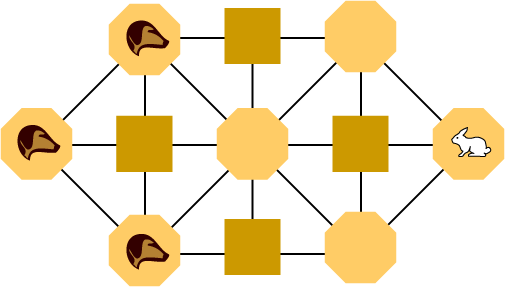
\includegraphics[width=.75\textwidth]{Hare_and_Hounds_board.png}
	\caption{The game board that Hare and Hounds is played on. The hare player
		starts on the right while the hounds player starts on the left.}
	\label{fig:board}
\end{figure}
